\documentclass[a4paper]{article}
\usepackage[letterpaper,top=2cm,bottom=2cm,left=3cm,right=3cm,marginparwidth=1.75cm]{geometry}
\usepackage[colorlinks=true, allcolors=blue]{hyperref}

\usepackage{wrapfig}
\usepackage{amsthm}
\usepackage{hyperref}
\usepackage{graphicx}
\usepackage{amsfonts}
\usepackage{csvsimple}

\title{Homework 3: Conjugate Gradient}
\author{Patryk Drozd}
\begin{document}
\date{}
\maketitle

\section*{Overview}

\section*{2.1}
\section*{2.2}
	
	
	\center
	\csvautotabular{q2out.csv}

	\begin{figure}[h!]
        \centering
        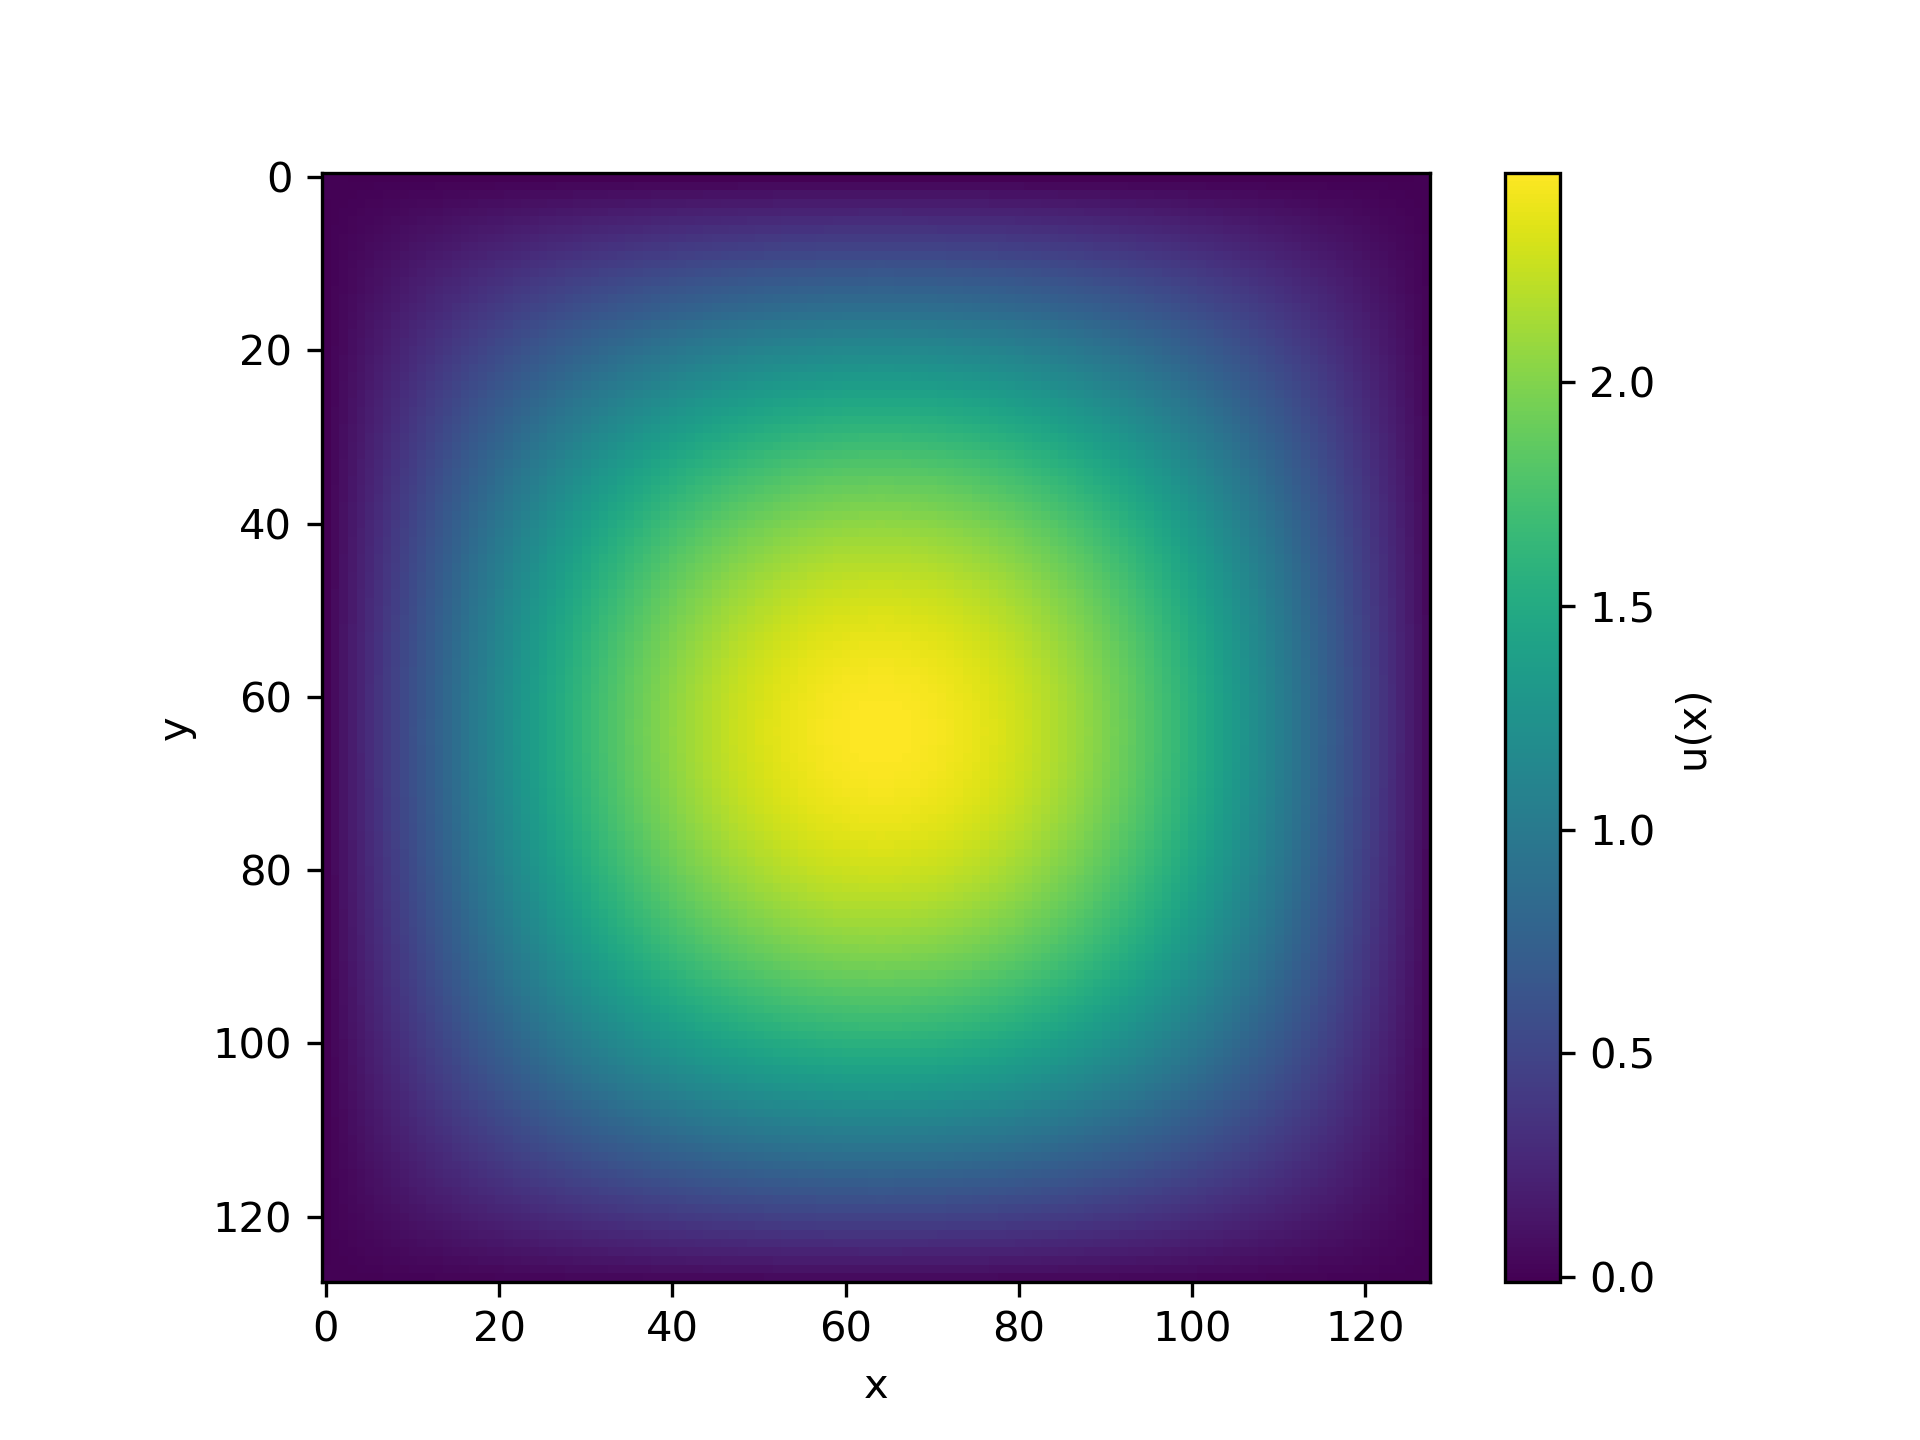
\includegraphics[width=.8\linewidth]{./q2plot.png}
        \caption{}
        \label{fig:q2_fig}
    \end{figure}	


\section*{2.3}
	
	\begin{figure}[h!]
        \centering
        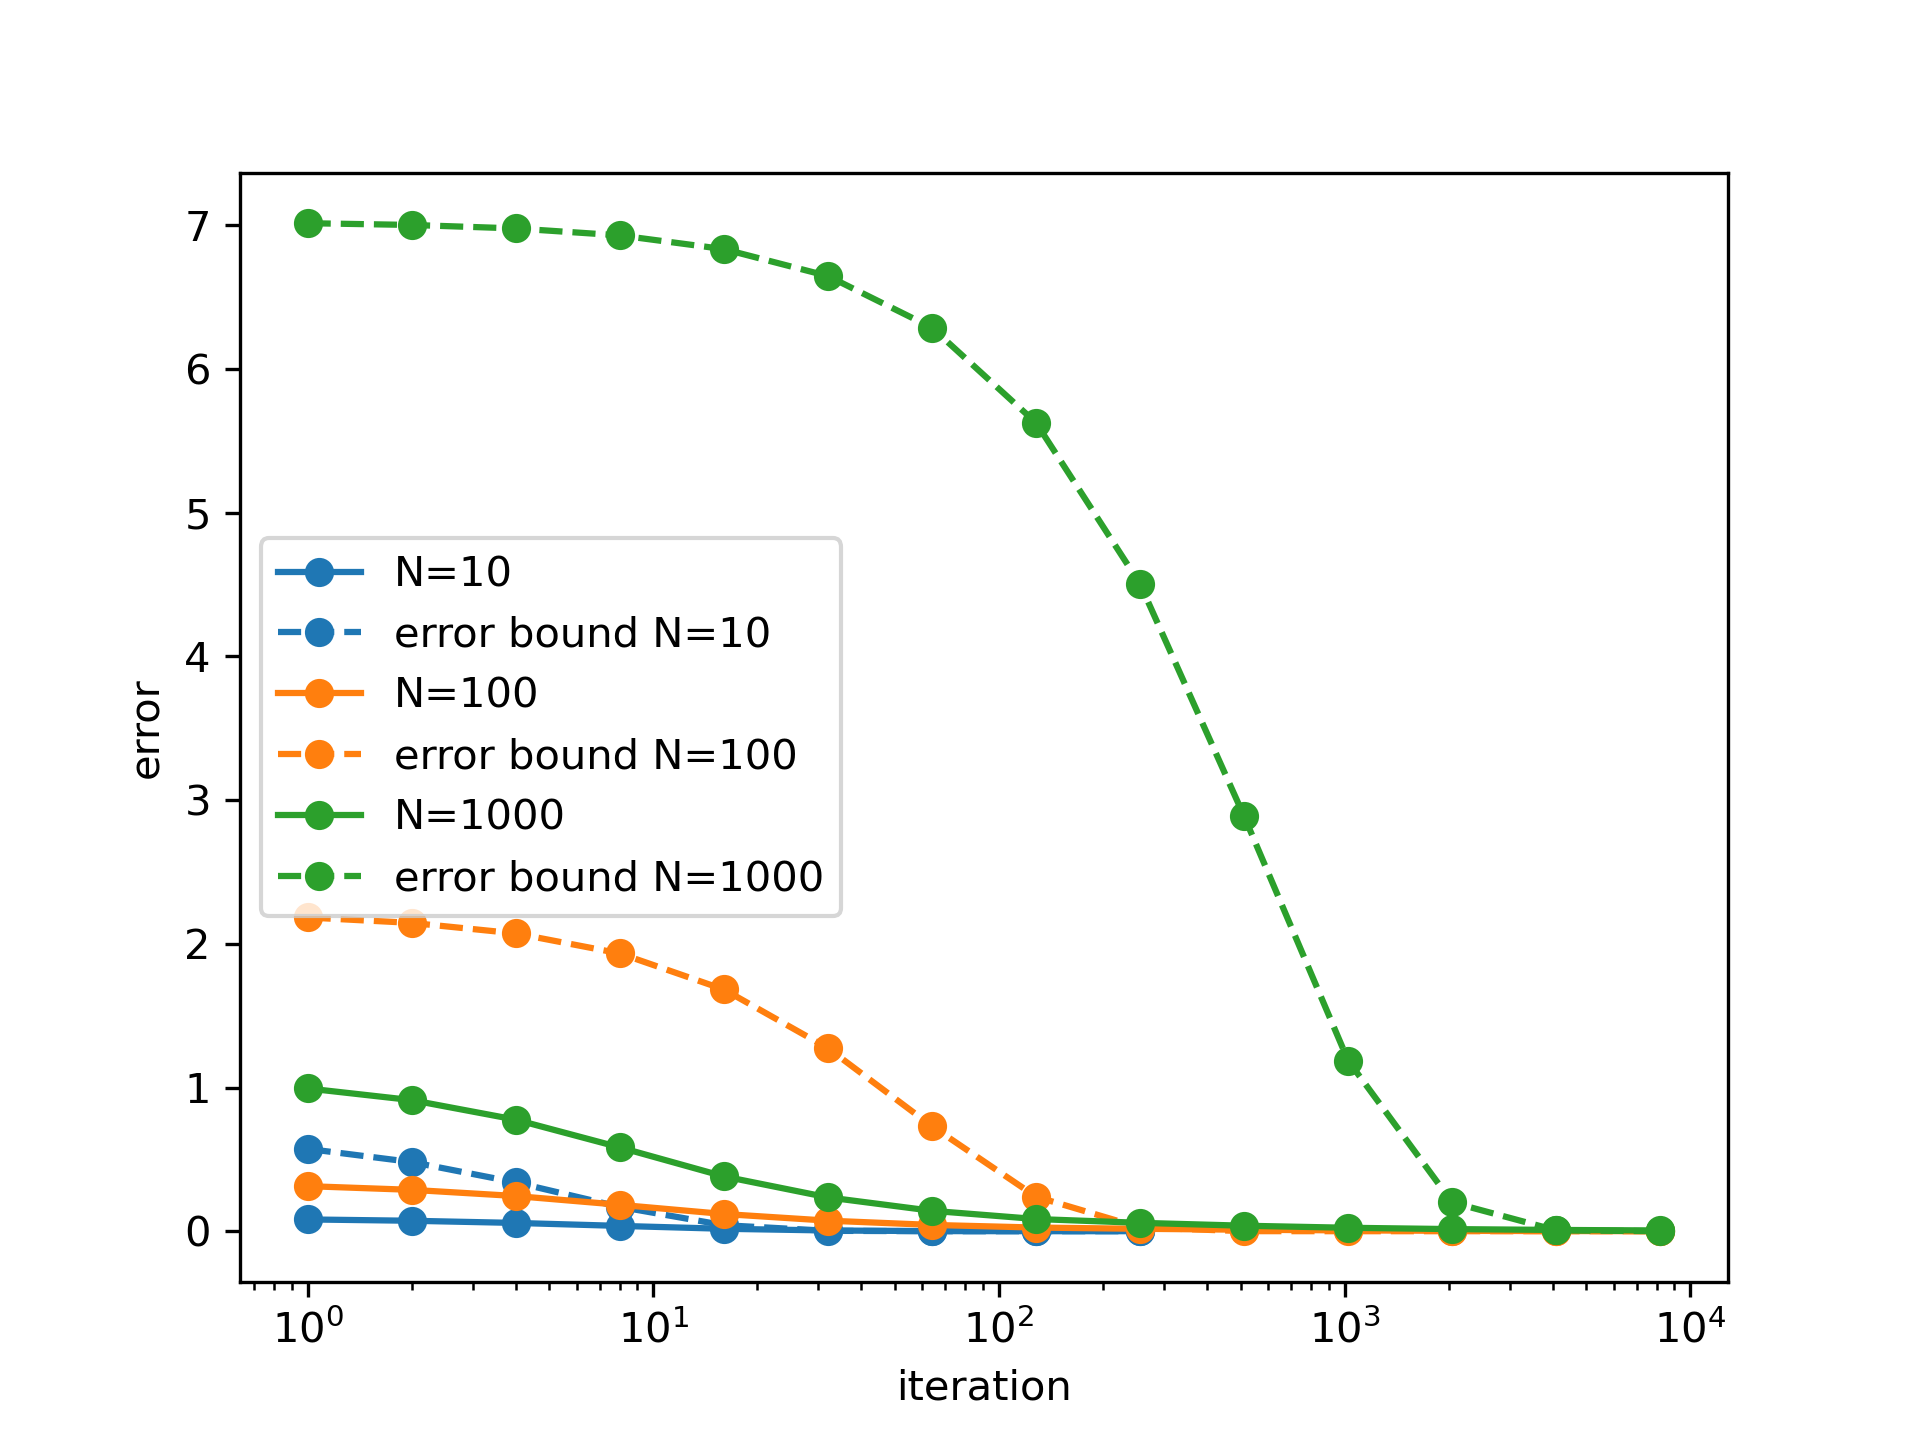
\includegraphics[width=.8\linewidth]{./q3plot.png}
        \caption{}
        \label{fig:q2_fig}
    \end{figure}	

\end{document}
